%
% chapter.tex -- Kapitel 2: Koordinaten und Tangentialvektoren
%
% (c) 2024 Prof Dr Andreas Müller
%
\chapter{Koordinaten und Tangentialvektoren
\label{chapter:koordinaten}}
\kopflinks{Koordinaten und Tangentialvektoren}
Die Bühne der Physik ist ein Raum von Punkten, in dem wir geometrische
Konstruktionen anwenden und zum Beispiel Bahnen von Körpern beschreiben
können.
Solche Beschreibungen verwenden immer mehr oder weniger speziell gewählte
Koordinatensysteme, die Punkte durch Koordinaten beschreiben.
Da die Koordinaten nur ein Werkzeug zur physikalischer Gegebenheiten
sind, muss es immer möglich sein, die zur Formulierung von Naturgesetzen
entwickelten Abstraktionen wie Kurven, Funktionen oder Vektoren zwischen
beliebigen Koordinatensystemen umzurechnen.
Ziel dieses Kapitels ist daher, eine für alle Arten von Koordinatensystemen
nützliche Notation zu entwickeln, die Umrechnung zwischen Koordinatensystemen
zu studieren und den Begriff des Tangentialvektors einzuführen.

%
% 1-koordinaten.tex -- Koordinaten
%
% (c) 2024 Prof Dr Andreas Müller
%
\section{Koordinaten
\label{buch:koordinaten:section:koordinaten}}
\kopfrechts{Koordinaten}
In diesem Abschnitt betrachten wir eine Punktmenge $X$, die mit
Koordinatensystemen ausgestattet werden soll.
Ohne das Koordinatensystem hat die Punktemenge keinerlei Struktur.
Um von stetigen Abbildungen zwischen solchen Mengen zu sprechen,
wird zum Beispiel ein Begriff der Nähe benötigt, mit dem die Konvergenz
von Folgen definiert werden kann.
Die Konstruktion eines Koordinatensystems ermöglicht, Punkte also
nahe beeinander zu betrachten, wenn sich ihre Koordinaten nur geringfügig
unterscheiden.

%
% Koordinatensystem
%
\subsection{Koordinatensystem}
%
% fig-koordinaten.tex
%
% (c) 2024 Prof Dr Andreas Müller
%
\begin{figure}
\centering
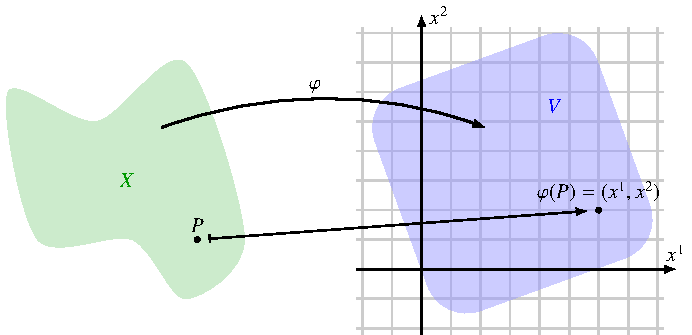
\includegraphics{chapters/020-koordinaten/images/koordinaten.pdf}
\caption{Ein Koordinatensystem auf der Punktmenge $X$ ist eine Abbildung 
$\varphi$ in den Koordinatenraum $V$, der eine Teilmenge von
$\mathbb{R}^n$ ist.
\label{buch:koordinaten:koordinaten:fig:koordinaten}}
\end{figure}
%
Ein $n$-dimensionales Koordinatensystem auf $X$ ordnet jedem Punkt 
ein $n$-Tupel von Koordinaten zu.
Aus erst später verständlichen Gründen bezeichnen wir die Koordinaten
mit hochgestellten Indizes, wir schreiben also $x^1,\dots,x^n$.
\index{Koordinaten}%
Eine Verwechslungsgefahr mit Exponenten besteht normalerweise nicht.
Falls die $k$-te Potenz der Koordinate $x^1$ berechnet werden soll, 
wird dies mit Klammern als $(x^i)^k$ geschrieben.
Ein Koordinatensystem ist also eine Abbildung
\[
\varphi
\colon
X\to \mathbb{R}^n
:
P \mapsto (x^1,\dots,x^n),
\]
wie sie in Abbildung~\ref{buch:koordinaten:koordinaten:fig:koordinaten}
dargestellt ist.
Jede einzelne Koordinate kann als Funktion $P\mapsto x^i(P)$ mit
reellen Werten betrachtet werden.

\begin{beispiel}
\label{buch:koordinaten:koordinaten:beispiel:kartpolar}
%
% fit-kartpolar.tex%
%
% (c) 2024 Prof Dr Andreas Müller
%
\begin{figure}
\centering
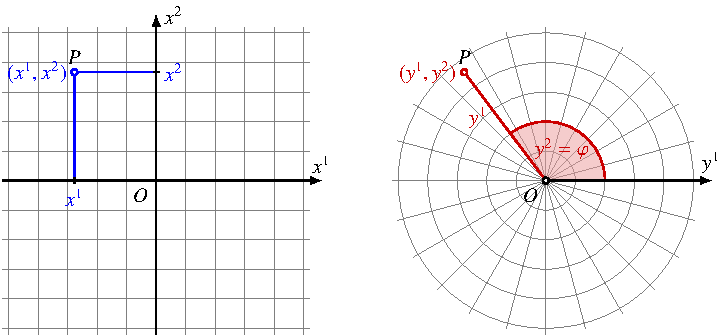
\includegraphics{chapters/020-koordinaten/images/kartpolar.pdf}
\caption{Zwei Koordinatensysteme für die Ebene:
kartesische (rechtwinklige) Koordinaten links und Polarkoordinaten
rechts.
Der gleiche Punkt $P$ wird gleichermassen durch die Koordinaten 
$(x^1,x^2)$ und $(y^1,y^2)$ beschrieben.
\label{buch:koordinaten:fig:kartpolar}}
\end{figure}

Die Punkte einer Ebene können einerseits mit dem {\em kartesischen}
Koordinatensystem mit den Koordinaten $(x^1,x^2)\in\mathbb{R}$ 
beschrieben werden und andererseits durch {\em Polarkoordinaten},
\index{Polarkoordinaten}%
\index{kartesische Koordinaten}%
die einen Punkt durch den Radius $y^1 = r$ und den Polarwinkel
\index{Polarwinkel}%
$y^2 = \varphi$ definieren (Abbildung~\ref{buch:koordinaten:fig:kartpolar}).

Die kartesischen Koordinaten können aus den Polarkoordinaten durch
\begin{equation}
\left.
\begin{aligned}
x^1 &= y^1\cos y^2 \\
x^2 &= y^1\sin y^2
\end{aligned}
\qquad
\right\}
\label{buch:koordinaten:koordinaten:eqn:polarkartumrechnung}
\end{equation}
berechnet werden.
\end{beispiel}

\begin{beispiel}
\label{buch:koordinaten:koordinaten:beispiel:kartkugel}
%
% fig-kartkugel.tex
%
% (c) 2024 Prof Dr Andreas Müller
%
\begin{figure}
\centering
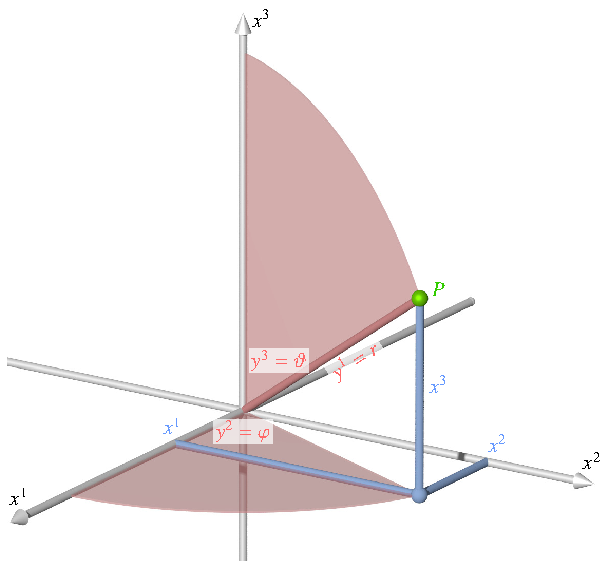
\includegraphics{chapters/020-koordinaten/images/kartkugel.pdf}
\caption{Kartesische Koordinaten ({\color{blue}blau}) und Kugelkoordinaten
({\color{darkred}rot}) für einen Punkt $P$ des dreidmensionalen Raumes.
\label{buch:koordinaten:koordinaten:fig:kartkugel}}
\end{figure}

Der dreidimensionale Raum kann sowohl durch {\em kartesische}
Koordinatentripel $(x^1,x^2,x^3)$ wie auch durch {\em Kugelkoordinaten}
\index{Kugelkoordinaten}%
beschrieben werden.
In Kugelkoordinaten ist ein Punkt durch die Entfernung $r=y^1$ vom
Nullpunkt, den Polarwinkel $y^2=\varphi$ seiner Projektion in die 
\index{Nullpunkt}%
$x^1$-$x^2$-Ebene und den Winkel $\vartheta$ zwischen der positiven
$x^3$-Achse und der Geraden durch Nullpunkt $O$ und den Punkt gegeben
(Abbildung~\ref{buch:koordinaten:koordinaten:fig:kartkugel}).
Die Umrechnung von Kugelkoordinaten in kartesische Koordinaten
\index{Kugelkoordinate}%
erfolgt mit
\begin{equation}
\left.
\begin{aligned}
x^1
&=
y^1 \cos y^2 \cos y^3 \\
x^2
&=
y^1 \sin y^2 \cos y^3 \\
x^3
&=
y^2 \cos y^3.
\end{aligned}
\qquad\right\}
\label{buch:koordinaten:koordinaten:eqn:kugelkartumrechnung}
\end{equation}
Man beachte, dass Punkte auf der $x^3$-Achse $y^3=0$ oder
$y^3=\pi$ und beliebigen Winkel $y^2\in\mathbb{R}$ haben.
Ohne zusätzliche Einschränkungen haben die Punkte auf der
$x^3$-Achse keine eindeutigen Kugelkoordinaten.
\end{beispiel}

Um die Struktur des Koordinatenraumes $\mathbb{R}^n$ auf die Menge
$X$ zu übertragen, müssen die Koordinatenabbildungen weiter eingeschränkt
werden.
Zunächst muss die Koordinatenabbildung bijektiv sein.
Dies bedeutet, dass jeder Punkt durch genau ein Koordinaten-$n$-Tupel
beschrieben wird.
Diese Bedingung ist in beiden Beispielen nicht erfüllt, da Tupel,
deren $y^2=\varphi$-Koordinaten sich um $2\pi$ unterscheiden, den
gleichen Punkt beschreiben.
Sie ist aber für genügend kleine Teilmengen des Raumes erfüllt.

Tatsächlich kann man nicht erwarten, zum Beispiel die Oberfläche einer
Kugel oder eines Torus in ihrer Gesamtheit eineindeutig auf Ebene
abzubilden.
Die Definition eines Koordinatensystems ist vorerst also nur geeignet,
eine Punktmenge lokal zu beschreiben.
Für eine globale Beschreibung wird es notwendig sein, verschiedene
Koordinatensysteme, die auf Teilen einer Menge definiert sind, zu
einem grösseren Ganzen zusammenzufügen.

Ausserdem muss die Menge $V=\varphi(X)$ der möglichen Koordinaten-$n$-Tupel
eine offene Menge in $\mathbb{R}^n$ sein.
Auch diese Bedingung ist in den Beispielen nicht erfüllt.
Die $y^1=r$-Koordinate nimmt alle Werte in
\[
\mathbb{R}_{\ge 0}
=
[0,\infty)
=
\{
y^1\in\mathbb{R}
\mid
y^1\ge 0
\}.
\]
\index{R@$\mathbb{R}_{\ge 0}$}%
Dies ist keine offene Menge, da die Punkte $(0,y^2)$ bzw.~$(0,y^2,y^3)$
ein Randpunkt des Wertebereichs der $y$-Koordinaten ist.
\index{offene Menge}%
\index{Randpunkt}%
Bei Kugelkoordinaten nimmt die Koordinate $y^3$ Werte im
abgeschlossenen Interval $[0,\pi]$ an, was zu weiteren Randpunkten
des Wertebereichs führen.

% XXX Beispiel zur Notwendigkeit der letzten Bedingung zeigen

%
% Koordinatenwechsel
%
\subsection{Koordinatenwechsel
\label{buch:koordinaten:koordinaten:subsection:koordinatenwechsel}}
In den Beispielen
\ref{buch:koordinaten:koordinaten:beispiel:kartpolar}
und
\ref{buch:koordinaten:koordinaten:beispiel:kartkugel}
wurden bereits Umrechnungsformeln zwischen den dort dargestellten
Koordinatensystemen ermittelt.
Seien etwas allgemeiner zwei Koordinatensysteme $x^1,\dots,x^n$
und $y^1,\dots,y^n$ auf der Punktmenge $X$ gegeben.
Sei $U$ die Menge der Koordinaten-$n$-Tupel, die Punkte von $X$
in den $x^i$-Koordinaten beschreiben, also die Bildmenge der
Koordinatenabbildung $\varphi$.
Dann ist die Umkehrabbildung $\varphi^{-1}$ auf $U$ definiert.

Sei weiter $\psi$ die Koordinatenabbildung für die $y^i$-Koordinaten
und $V$ der zugehörige Wertebereich.
Die Zusammensetzung
\[
\psi
\circ
\varphi^{-1}
\colon
U\to V\subset\mathbb{R}^n
:
(x^1,\dots,x^n)
\mapsto
(y^1,\dots,y^n)
\]
ist die Koordinatenumrechnung vom $x^i$-Koordinatensystem in
das $y^i$-Koordinatensystem, eine Abbildung von $U$ in $V\subset\mathbb{R}^n$.

% XXX Koordinatenwechsel-Abbildung

Die Koordinatenwechsel-Abbildung ist umkehrbar, da sowohl $\varphi$
als auch $\psi$ umkehrbar sind.
\index{Koordinatenwechsel}
Die Umkehrabbildung ist die Abbildung
\[
(\psi\circ\varphi^{-1})^{-1}
=
\varphi\circ\psi^{-1}
\colon
V\to W \subset \mathbb{R}^n.
\]

%
% Stetigkeit
%
\subsubsection{Stetigkeit}
Die Koordinatenabbildungen $\varphi$ ermöglicht, auf der Menge
$X$ zu definieren, was eine konvergente Folge ist.
Die Punkte $P_k\in X$ konvergieren genau dann gegen den Punkt $P$,
wenn die Bildpunkte $\varphi(P_k)$ in $U$ gegen $\varphi(P)$
konvergieren.

Eine weitere Koordinatenabbildung $\psi\colon X\to V$ definiert einen
weiteren Begriff der Konvergenz von Punktfolgen in $X$.
Die Eigenschaft einer Folge, zu konvergieren, sollte nicht davon 
abhängig sein, in welchen Koordinaten der Grenzwert berechnet
werden soll.
Für jedes Koordinatensystem sollte sich der gleiche Begriff der
Konvergenz von Folgen ergeben.
Dies schränkt die Menge der zulässigen Koordinatensysteme ein.

Zwei Koordinatensysteme $\varphi$ und $\psi$ führen auf den gleichen
Konvergenzbegriff, wenn für jede Folge $P_k\in X$ die Folgen
\[
x_k=\varphi(P_k)\in V
\qquad\text{und}\qquad
y_k=\psi(P_k)\in W
\]
beide konvergent oder beide nicht konvergent sind.
Dies trifft genau dann zu, wenn die Koordinatenwechselabbildungen
$\psi\circ\varphi^{-1}$ in jedem Punkt stetig sind.

Die Konvergenz einer Folge in $\mathbb{R}^n$ wird durch das Verhalten
der Entfernung
\[
d(P,Q)
=
|x(P)-x(Q)|
\]
von Punkten bestimmt.
Die Funktion $d$ heisst auch die vom Koordinatensystem induzierte 
{\em Metrik}.
\index{Metrik}%
Eine Folge $P_k$ konvergiert gegen $P$, wenn es für jedes $\varepsilon>0$
eine Zahl $N$ gibt derart, dass der Abstand $d(P,P_k)<\varepsilon$, wenn
$k>N$ ist.
Der Begriff des Abstandes von Punkten lässt sich mit der Koordinatenabbildung
nicht auf die Menge $X$ übertragen, da die Abstände je nach Koordinatensystem
verschieden sein können.
Dies ist aber auch nicht nötig, denn Konvergenz verlangt nur, dass genügend
kleine Abstände in einem Koordinatensystem auch genügend klein sind in jedem
anderen Koordinatensystem.
Die Koordinatenwechselabbildung $\psi\circ\varphi^{-1}$  muss daher die
Bedingung erfüllen, dass es für jedes $\varepsilon>0$ ein $\delta>0$ gibt,
dass 
\[
|y(P)-y(Q)| < \varepsilon
\]
für alle Paare von Punkten $P$ und $Q$ mit $|x(P)-x(Q)| < \delta$
gilt.
Dies ist aber die Definition einer stetigen Abbildung.

\begin{definition}[offene Menge in $X$]
\label{buch:koordinaten:koordinaten:definition:offenemenge}
Eine Menge $U\subset X$ heisst eine {\em offene Menge}, wenn es für jeden Punkt
\index{offene Menge}%
\index{Menge, offen}%
$P\in X$ und für jedes Koordinatensystem $\varphi\colon X\to V$
ein $\varepsilon >0$ gibt derart, dass die Menge
\[
U_{P,\varphi}
=
\varphi^{-1}\bigl(
\{
x\in V
\mid
|x-\varphi(P)|<\varepsilon
\}
\bigr)
\]
in $U$ enthalten ist: $U_{P,\varphi}\subset U$.
\end{definition}

Die Definition transportiert die Idee einer kleinen Umgebung
eines Punktes mithilfe der Koordinatenabbildung von der Bildmenge
$V\subset \mathbb{R}^n$ auf die Menge $X$.
Damit sich daraus ein konsistenter Begriff der kleinen Umgebung 
ergibt, müssen verschiedene Koordinatensysteme die gleichen
kleinen Umgebungen erzeugen.
Dies wird durch die folgende Definition sichergestellt.

\begin{definition}[stetige Struktur]
\label{buch:koordinaten:koordinaten:definition:stetigestruktur}
\index{stetige Struktur}%
\index{Struktur!stetig}%
Eine {\em stetige Struktur} auf der Punktemenge $X$ ist eine mit
der Indexmenge $I$ indizierte Familie
\[
\varphi_\alpha\colon X\to V_\alpha \subset \mathbb{R}^n,
\]
$\alpha\in I$,
von Koordinatensystemen auf der Menge $X$ derart, dass die
Koordinatenwechselabbildungen
\[
\varphi_{\beta}\circ\varphi_\alpha^{-1}
\colon
V_\alpha \to V_\beta
\]
stetige Abbildungen für alle $\alpha,\beta\in I$ sind.
\end{definition}

Mit jedem Koordinatenwechsel ist auch die Umkehrabbildung ein
Koordinantenwechsel.
Die Koordinatenwechsel sind also alle umkehrbare stetige Abbildungen,
oder {\em Homöomorphismen}.
\index{Homoomorphismus@Homöomorphismus}%

Will man ein neues Koordinatensystem auf $X$ verwenden, muss es so
gewählt werden, dass es mit allen bereits verwendeten Koordinatensystemen
verträglich ist.
Die Koordinatenwechsel von und zum neuen Koordinatensystem müssen
alle stetig sein.

%
% Stetige Funktionen auf X
%
\subsubsection{Stetige Funktionen auf $X$}
Sei jetzt $f\colon X\to\mathbb{R}$ eine reellwertige Funktion.
Ohne ein Koordinatensystem ist nicht klar, was es heissen soll, dass die
Funktion $f$ stetig ist.
Mit Hilfe eines Koordinatensystems $\varphi\colon X\to V$ kann man die
Funktion $f$ jetzt auch in Koordinaten schreiben.
Dazu bildet man die Funktion
\[
f_\varphi
=
f\circ \varphi^{-1}
\colon
V
\to
\mathbb{R}
:
(x^1,\dots,x^n)
\mapsto
f(\varphi^{-1}(x^1,\dots,x^n))
=
f(x^1,\dots,x^n).
\]
Eine Funktion $f$ heisst stetig, wenn die in $x$-Koordinaten geschriebene
Funktion $f(x^1,\dots,x^n)$ eine stetige Funktion ist.
Wählt man ein anderes Koordinatensystem $\psi\colon X\to W$ einer
stetigen Struktur auf $X$, dann ist der Koordinatenwechsel
$\varphi\circ\psi^{-1}$ ein Homöomorphismus, insbesondere ist 
\[
f_\psi
=
f\circ\psi^{-1}
=
\underbrace{f\circ\varphi^{-1}}_{\displaystyle f_\varphi\mathstrut}
\circ
\underbrace{\varphi\circ\psi^{-1}}_{\displaystyle
\hbox to6pt{\rlap{\text{Koordinatenwechsel\strut}}\hfill}}
\colon
W\to \mathbb{R}
\]
genau dann stetig, wenn auch $f_\varphi$ stetig ist.
Eine stetige Struktur auf $X$ ermöglicht also insbesondere auch,
auf konsistente Weise über Stetigkeit von rellwertigen Funktionen
auf $X$ zu sprechen.

%
% Differenzierbarkeit
%
\subsubsection{Differenzierbarkeit}
Für eine beliebige Punktmenge $X$ ist es im Allgemeinen nicht sinnvoll,
von differenzierbaren Funktionen zu sprechen.
\index{differenzierbar}%
Die Existenz der Ableitung $f'(x_0)$ einer Funktion im Punkt $x_0$
basiert darauf, dass es eine lineare Ersatzfunktion
\index{lineare Ersatzfunktion}%
\begin{equation}
f(x) = f(x_0) + f'(x_0)\cdot (x-x_0)+o(x-x_0)
\label{buch:koordinaten:koordinaten:eqn:linersatz}
\end{equation}
gibt.
Die Notation $o(t)$ bezeichnet eine Funktion mit der Eigenschaft
\[
\lim_{t\to 0} \frac{o(t)}{t}=0
\]
(Lambert-$o$-Notation).
\index{Lambert-o-Notation@Lambert-$o$-Notation}%
\index{o-Notation@$o$-Notation}%
Die Darstellung~\eqref{buch:koordinaten:koordinaten:eqn:linersatz}
ist nur sinnvoll, wenn der Definitions- wie auch der Wertebereich
Teilmengen von $\mathbb{R}$ sind.

Eine Funktion $f\colon X\to \mathbb{R}$ kann in einem Koordinatensystem
$\varphi\colon X\to V\subset\mathbb{R}^n$ als Funktion
\[
f_\varphi
\colon
V\to\mathbb{R}
:
(x^1,\dots,x^n)
\mapsto
f\circ\varphi^{-1}(x^1,\dots,x^n)
\]
der Koordinaten $x^i$ geschrieben werden.
Damit ist die Voraussetzung geschaffen, von den Ableitungen von $f$
nach jeder beliebigen Koordinate zu sprechen.
Die {\em partielle Ableitung} von $f$ nach der Koordinaten $x^i$ im
Koordinatensystem $\varphi$ ist
\begin{equation}
\frac{\partial f}{\partial x^i}
=
\frac{\partial f_\varphi}{\partial x^1}(x^1,\dots,x^n)
=
\lim_{h\to 0}
\frac{f_\varphi(x^1,\dots,x^i+h,\dots, x^n)-f(x^1,\dots,x^n)}{h}.
\label{buch:koordinaten:koordinaten:eqn:partabl}
\end{equation}
Bei der Ableitung werden alle Koordinaten ausser der Koordinaten $x^i$
konstant gehalten.

Der Ausdruck~\eqref{buch:koordinaten:koordinaten:eqn:partabl} ist ganz
explizit von der Wahl des Koordinatensystems abhängig.
Sei $\psi\colon X\to W$ ein weiteres Koordinatensystem, dann lassen sich
die Koordinaten $x^i$ des Koordinatensystems $\varphi$ in die 
Koordinaten $y^k$ des Koordinatensystems $\psi$ umrechnen.
Die Koordinate $y^k$ ist eine reellwertige Funktion auf $X$, wir
können daher auch die partiellen Ableitungen
\[
\frac{\partial y^k}{\partial x^i}(x^1,\dots,x^n)
\]
bilden.
Aus der Kettenregel können jetzt die partiellen Ableitung bezüglich
\index{Kettenregel}%
der Variablen $y^k$ durch die partiellen Ableitungen bezüglich der
Variablen $x^i$ als
\begin{align*}
\frac{\partial}{\partial x^i}
(f\circ\psi^{-1})\circ (\psi\circ\varphi^{-1})(x^1,\dots,x^n)
&=
\sum_{k=1}^n
\frac{\partial f\circ\psi^{-1}}{\partial y^k}(y^1,\dots,y^n)
\cdot
\frac{\partial y^k}{\partial x^i}(x^1,\dots,x^n)
\end{align*}
ausgedrückt werden.

\begin{definition}[Jacobi-Matrix]
Die Matrix
\[
J
=
\frac{\partial(y^1,\dots,y^n)}{\partial(x^1,\dots,x^n)}
=
\bgroup
\renewcommand\arraystretch{1.8}
\begin{pmatrix}
\displaystyle\frac{\partial y^1}{\partial x^1}&\dots&\displaystyle\frac{\partial y^1}{\partial x^n}\\
\vdots&\ddots&\vdots\\[-2pt]
\displaystyle\frac{\partial y^n}{\partial x^1}&\dots&\displaystyle\frac{\partial y^n}{\partial x^n}\\
\end{pmatrix}
\egroup
\]
mit den Matrixeinträgen
\[
J_{ki}
=
\frac{\partial y^k}{\partial x^i}(x^1,\dots,x^n)
\]
heisst die {\em Jacobi-Matrix} der Funktionen $y^k(x_1,\dots,x_n)$,
$k=1,\dots,n$.
\index{Jacobi-Matrix}%
\index{J}
\end{definition}

Die Umrechnung der partiellen Ableitungen zwischen verschiedenen
Koordinatensystemen erfolgt also mit Hilfe der Jacobi-Matrix der
Koordinatentransformation.

\begin{definition}
Ein Koordinatenwechsel $\psi\circ\varphi^{-1}$ heisst
\index{Koordinatenwechsel}%
{\em stetig differenzierbar}, wenn die Jacobi-Matrix $J$
stetig ist.
\end{definition}

Die Eigenschaft der Differenzierbarkeit einer Funktion sollte wie
im Falle der Stetigkeit nicht von der Wahl eines Koordinatensystems
abhängen.
Das kann nur funktionieren, wenn die Umrechnung zwischen verschiedenen
Koordinatensystemen immer möglich ist.
Dazu muss die Jacobi-Matrix in jedem Punkt des Koordinatensystems
definiert sein.
Dies schränkt die Wahl der zulässigen Koordinatensysteme weiter ein.

\begin{definition}[differenzierbare Struktur]
\label{buch:koordinaten:koordinaten:definition:diffbareestruktur}
Eine {\em differenzierbare Struktur} auf $X$ ist eine stetige Struktur,
\index{differenzierbare Struktur}%
\index{Struktur!differenzierbar}%
deren Koordinatenwechsel stetig differenzierbar sind.
\end{definition}


%
% 2-tangentialvektoren.tex -- Tangentialvektoren
%
% (c) 2024 Prof Dr Andreas Müller
%
\section{Tangentialvektoren
\label{buch:koordinaten:section:tangentialvektoren}}
\kopfrechts{Tangentialvektoren}
Das elektrische Feld übt auf eine Testladung eine Kraft aus, die
proportional zur Ladung ist.
\index{Testladung}%
\index{Kraft}%
Diese Kräfte stellt man sich gerne als ein Vektorfeld vor, doch
in welchem Raum sind diese Vektoren zu finden?
Die Kraft verursacht eine Beschleunigung und verändert damit 
die Geschwindigkeit.
\index{Geschwindigkeit}%
\index{Beschleunigung}%
%
% fig-tangentialvektoren.tex
%
% (c) 2025 Prof Dr Andreas Müller
%
\begin{figure}
\centering
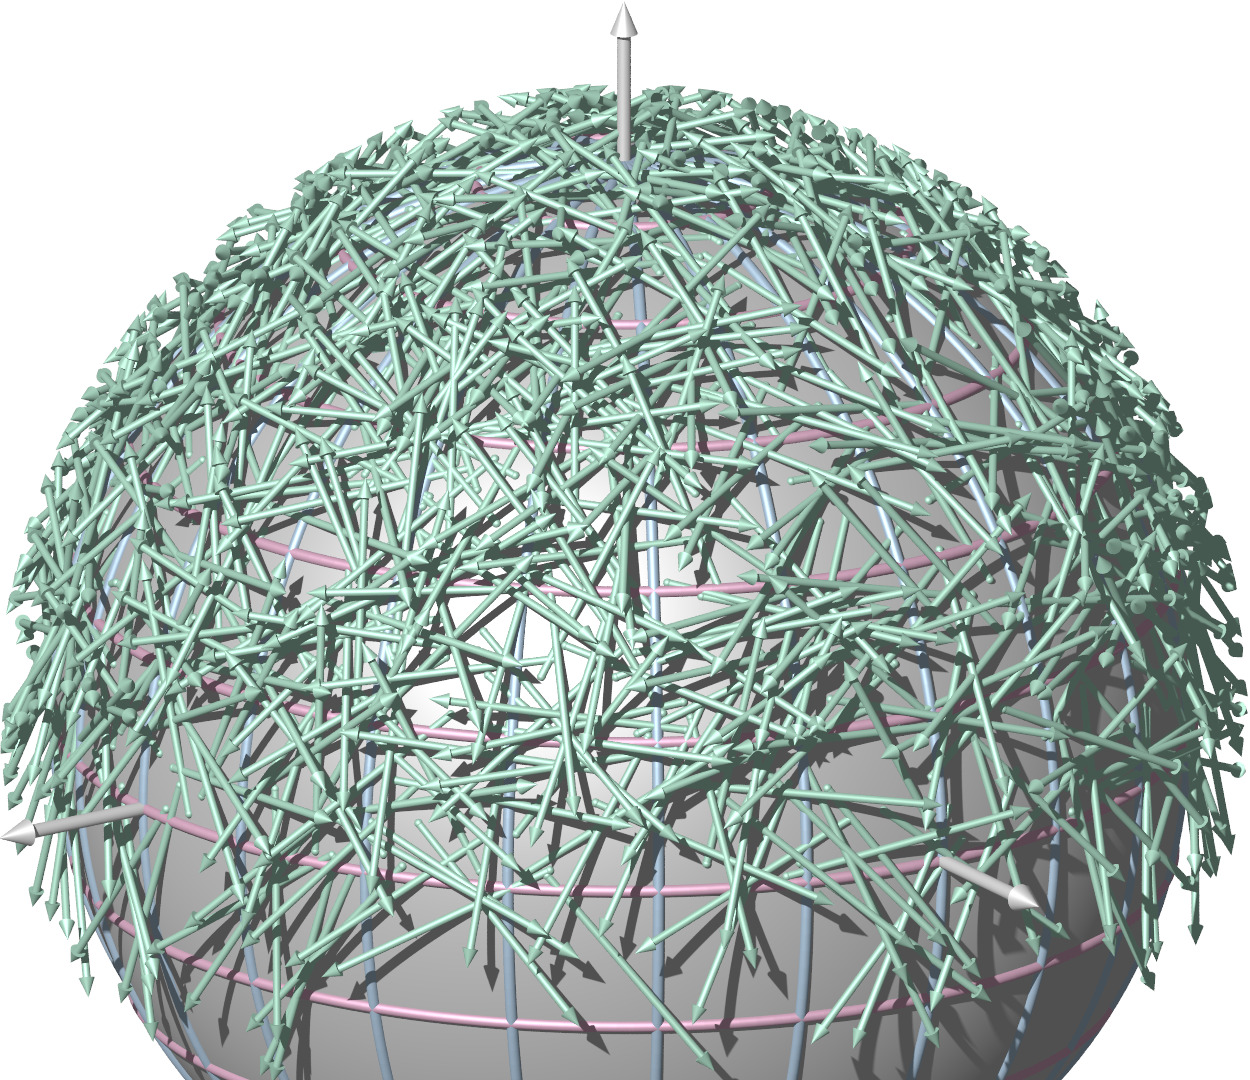
\includegraphics[width=10cm]{chapters/020-koordinaten/images/tangentialvektoren.jpg}
\caption{Darstellung von tausend Tangentialvektoren an die Nordhalbkugel.
Ganz offensichtlich sind die Tangentialvektoren nicht Teil der Kugel.
\label{buch:koordinaten:fig:tangentialvektoren}}
\end{figure}
%
Als erstes muss daher der Geschwindigkeitsvektor konstruiert werden,
der tangential an die Bahnkurve der Testladung verläuft.
An dieser naheliegenden und üblichen Darstellung ist aber eigentlich
falsch, dass der Geschwindigkeitsvektor gar nicht im gleichen Raum
dargestellt werden kann
(Abbildung~\ref{buch:koordinaten:fig:tangentialvektoren}).
Die Masseinheit der Komponenten des Geschwindigkeitsvektors ist
[Länge/Zeit], während die Koordinaten die Masseinheit [Länge] haben.
\index{Masseinheit}%
Solange man das Koordinatensystem und damit die Masseinheiten nicht
wechselt, mag die Konfusion in Grenzen bleiben.
Da aber alle Gesetzmässigkeiten auf eine koordinatensystemunabhängige
Art formuliert werden müssen, bedarf auch das Konzept des Tangentialvektors
einer Reevaluation.

%
% Kurven
%
\subsection{Kurven}
Für ein kartesisches Koordinatensystem in der Ebene ist klar, welche
Richtung man den Koordinatenachsen zuordnen kann.
Es ist üblich, die Koordinatenachsen als Vektoren in der Ebene
zu zeichnen.
Die Idee einer geraden Koordinatenachse ist nicht mehr anwendbar,
wenn beliebige Koordinatensysteme verwendet werden sollen.
Bei der Umrechnung zwischen Koordinatensystemen entstehen unweigerlich
gekrümmte Koordinatenlinien.
Es braucht also etwas mehr Sorgfalt, die Idee der {\em Richtung}
Koordinatenunabhängig zu definieren.

\subsubsection{Differenzierbare Kurven}
Im Folgenden gehen wir on einer Menge $Y$ mit einer $n$-dimensionalen
differenzierbaren Struktur aus.
Statt uns auf die in der Einleitung angedeuteten gekrümmten
Koordinatenlinien zu beschränken, möchten wir beliebige Kurven
definieren.
Kurven sehen in der Umgebung eines Punktes wie die reelle Achse
$\mathbb{R}$ aus.
Tatsächlich können wir jedes Intervall $X=(a,b)\subset\mathbb{R}$ als
eine Menge mit einer differenzierbaren Struktur betrachten, indem
wir die Einbettung
\[
\varphi
\colon
X=(a,b) \hookrightarrow \mathbb{R}
:
x\mapsto x
\]
als Koordinatensystem verwenden (Der ``Haken'' am Abbildungspfeil
soll die Einbettung symbolisieren).
Die Koordinatenwechselabbildung zu einem alternativen Koordinatensystem
auf dem Intervall ist eine streng monoton wachsende, differenzierbare
Funktion, deren Ableitung nirgends verschwindet.
In einem Punkt $x_0\in (a,b)$ sind Koordinatenwechsel daher sehr
einfach: Sie sind nur von 0 verschiedene Zahlen.
Diese Einfachheit erlaubt uns, zur Vereinfachung der Notation die Menge
$(a,b)$ mit den Koordinatenwerten zu identifizieren.

\begin{definition}[differenzierbare Kurve]
Eine {\em differenzierbare Kurve}
\index{differenzierbare Kurve}%
\index{Kurve, differenzierbar}%
ist eine differenzierbare Abbildung
\[
\gamma
\colon
X = (a,b) \to Y
:
t \mapsto \gamma(t).
\]
\end{definition}

Durch Zusammensetzen der Abbildung $\gamma$ mit einem Koordinatenssystem
$\varphi\colon X\to \mathbb{R}^n$ entsteht eine Abbildung 
\[
\varphi\circ\gamma
\colon
X=(a,b) \to \mathbb{R}^n
:
t \mapsto (\varphi^1\circ \gamma(t),\dots,\varphi^n\circ\gamma(t)),
\]
wobei jede Koordinate $\varphi^i\circ\gamma(t) = \varphi^i(\gamma(t))$
eine differenzierbare Funktion von $t$ ist.

\begin{beispiel}
Die Menge $Y=\mathbb{R}^2$ hat eine differenzierbare Struktur gegeben durch
das kartesische Koordinatensystem
\[
\varphi
\colon
Y\to\mathbb{R}^2
:
(x,y)\mapsto (x,y).
\]
Die Kurve 
\[
\gamma
\colon
\mathbb{R}\to Y
:
t\mapsto (\cos t, \sin t)
\]
ist der Einheitskreis in der Ebene.

Koordinatenwechsel auf dem Urbildbereich $(-\infty,\infty)$ sind durch
Funktionen $f\colon\mathbb{R}\to\mathbb{R}$ gegeben, deren Ableitung
nirgends verschwindet.
Nach dem Koordinatenwechsel ist die Kurven durch die Parametrisierung
\[
t \mapsto (\cos f(t),\sin f(t))
\]
gegeben.

Statt der kartesischen Koordinaten kann man mindestens auf der Teilmenge
$Y=X\setminus (0,0)$ Polarkoordinaten mit der Koordinatenabbildung $\psi$
verwenden.
Die Koordinatenumrechnung von Polarkoordinaten in kartesische Koordinaten
ist
\[
(\varphi, r) \mapsto (r\cos\varphi,r\sin\varphi)
\]
mit der Umkehrung
\[
(x,y) \mapsto \Bigl(\arctan\frac{y}{x},\sqrt{x^2+y^2}\Bigr),
\]
wobei die $\arctan$-Funktion etwas erweitert werden muss, wie es die
in den meisten Programmierbibliotheken durch die Funktion \texttt{atan2}
gemacht wird.

In Polarkoordinaten bekommt die Kurve $\gamma$ die Form
\[
t\mapsto \psi\circ\gamma(t)
=
(t, 1).
\]
Die zweite Koordinaten ist konstant und damit ganz offensichtlich 
differenzierbar.
Die erste Koordinate hat die Ableitung $1$.
\end{beispiel}

Eine Kurve in $Y$ ist also eine Abbildung $X\to Y$.
Sowohl in $X$ wie auch in $Y$ können beliebige Koordinatensysteme
gewählt werden.
Es ist nur sinnvoll über Objekte zu sprechen, welche in dem
Sinne unabhängig sind von der Wahl des Koordinatensystems, dass
auch Umrechnungsformeln zwischen den Koordinatensystemen bereitgestellt
sind.

% XXX Ableitung der Koordinaten

% XXX Koordinatenwechsel und Ableitung


\subsubsection{Tangentiale Kurven}
Das Beispiel illustriert, dass der Begriff der ``Richtung'' einer
Koordinatenachse nicht sinnvoll sein kann.
Im Wertebereich der Koordinatensysteme unterscheidet sich das Bild
der Kurve $\gamma$ grundsätzlich.
Im Koordinatensystem ist $\varphi\circ\gamma$ eine gekrümmte Kurve,
während sie im Polarkoordinatensystem in der Umgebung des Punktes
$(1,0)$ die Gerade $r=1$ ist.
Die Kurve durch einen Punkt von $Y$ kann also keine koordinatenunabhängig
Bedeutung haben, aber für die Richtung der Kurve in einem Punkt ist
dies möglich.
Es muss daher definiert werden, wann zwei Kurven die gleiche Richtung
in einem gemeinsamen Punkt haben.


%
% fig-kurve.tex
%
% (c) 2024 Prof Dr Andreas Müller
%
\begin{figure}
\centering
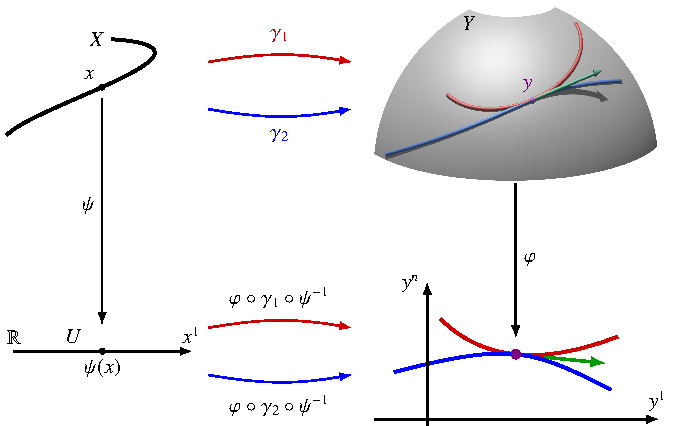
\includegraphics{chapters/020-koordinaten/images/kurve.pdf}
\caption{Die Kurven $\gamma_1$ und $\gamma_2$ sind tangential im
Punkt $y$, wenn $\gamma_1(x)=y=\gamma_2(x)$ und ausserdem die
Ableitungen der Zusammensetzungen $\varphi\circ\gamma_i\circ\psi^{-1}$
in $\psi(x)$ übereinstimmen.
Es ist nicht sinnvoll, von einem Tangentialvektor ``in $Y$'' (grün,
oben rechts) zu sprechen, erst durch das Koordinatensystem kann
das Konzept des Tangentialvektors konsistent definiert werden.
\label{buch:koordinaten:tangentialvektoren:fig:kurve}}
\end{figure}
%

\begin{definition}[tangentiale Kurven]
\index{tangentiale Kurven}%
Zwei Kurven $\gamma_i\colon X\to Y$, $i=1,2$, sind
{\em tangential} im Punkt $y\in Y$, wenn
$\gamma_i(x) = y$, $i=1,2$, und
in jeder Karte
$\varphi\colon Y\to\mathbb{R}^n$ und für die Parametrisierung
$\psi\colon X\to \mathbb{R}$ mit Parameter $x^1\in\mathbb{R}$ 
im Punkt $\psi(x)$ die Ableitungen der Abbildungen
\[
\varphi
\circ
\gamma_i
\circ
\psi^{-1}
\colon
U\to\mathbb{R}^n
\]
übereinstimmen, d.~h.
\begin{equation}
\frac{d}{dx^1}
\bigl(\varphi\circ\gamma_1\circ\psi^{-1}\bigr)(\psi(x))
=
\frac{d}{dx^1}
\bigl(\varphi\circ\gamma_2\circ\psi^{-1}\bigr)(\psi(x))
\label{buch:koordinaten:tangentialvektoren:eqn:tangential}
\end{equation}
für $x^1=\psi(x)$.
\end{definition}

Kurven sind also tangential in einem Punkt, wenn sie sich in jedem
Koordinatensystem mit der gleichen momentanen Geschwindigkeit
\index{momentane Geschwindigkeit}%
durch den Punkt im Koordinatenraum bewegen.
Die Abbildung~\ref{buch:koordinaten:tangentialvektoren:fig:kurve}
macht auch deutlich, dass es nicht sinnvoll ist, von einem
Tangentialvektor im Punkt $y$ an die Kurven ``in $Y$'' zu sprechen.
Der grün eingezeichnete Tangentialvektor ist nicht Teil von $Y$.
Er hängt von der Art der für die graphische Darstellung notwendigen
Einbettung von $Y$ in den dreidimensionalen Raum ab.
Eine rein geometrische Definition des Tangentialvektors ist also
nicht möglich.
Erst im Koordinatensystem, also nach der Abbildung mit $\varphi$,
entsteht ein Tangentialvektor, mit dem man in $\mathbb{R}^n$
rechnen kann, doch dieser Tangentialvektor hängt notwendigerweise
vom Koordinatensystem ab.
Es muss daher zusätzlich geklärt werden, wie sich der Tangentialvektor
ändert, wenn man ein anderes Koordinatensystem verwendet.

%
% Tangentialvektoren
%
\subsection{Tangentialvektoren}
Die Eigenschaft von Kurven, im Punkt $y$ tangential zu sein, ist
eine Äquivalenzrelation.
In einem Koordinatensystem haben die tangentiale Kurven gemäss
Abbildung~\ref{buch:koordinaten:tangentialvektoren:fig:kurve}
den grünen Tangentialvektor \emph{im Koordinatensystem} gemeinsam.
Die folgende, sehr abstrakte Definition eines Tangentialvektors
von $Y$ ist unabhängig von einer Einbettung von $Y$ in einen
grösseren Raum für Darstellungszwecke.

\begin{definition}[Tangentialvektor]
\label{buch:koordinaten:tangentialvektoren:def:tangentialvektor}
\index{Tangentialvektor}%
Ein Tangentialvektor $V$ im Punkt $y\in Y$ ist die Menge aller Kurven, die
im Punkt $y$ tangential sind.
In einem Koordinatensystem $\varphi$ ist der Tangentialvektor an die Kurve
$\gamma$ durch die Komponenten
\[
u^i
=
\frac{d}{dx^1} \varphi^i(\gamma(\psi(x^1))) \bigg|_{x^1 = \psi(x)}
\]
gegeben.
Der Tangentialvektor an die Kurve $\gamma$ an der Stelle $x$
wird auch als $T_x\gamma\cdot e_1$ bezeichnet.
\end{definition}

Verwendung eines anderen Koordinatensystems $\varphi'$ anstelle von
$\varphi$ bedeutet, dass die Komponenten des Tangentialvektors
an die Kurve mit der Koordinatentransformation
$g=\varphi'\circ\varphi^{-1}$ umgerechnet werden müssen.
Im neuen Koordinatensystem sind die Komponenten
\begin{align}
u^{\prime i}
&=
\frac{d}{dx^1}
\varphi^{\prime i}(\gamma(\psi^{-1}(x^1))) \bigg|_{x^1=\psi(x)}
\notag
\\
&=
\frac{d}{dx^1}
(\varphi'\circ\varphi^{-1})^i\circ \varphi\circ\gamma\circ\psi^{-1}(x^1)
\bigg|_{x^1=\psi(x)}
\notag
\\
&=
\frac{d}{dx^1} g^i\circ(\varphi\circ\gamma\circ\psi^{-1})(x^1)
\bigg|_{x^1=\psi(x)}
\notag
\\
&=
\sum_{k=1}^n
\frac{\partial g^i}{\partial y^k}(\varphi(y))
\cdot
\frac{d}{dx^1}\varphi^k(\circ(\psi^{-1})) 
\bigg|_{x^1=\psi(x)}
\notag
\\
&=
\sum_{k=1}^n
\frac{\partial g^i}{\partial y^k}(\varphi(y))
\cdot
u^k.
\label{buch:koordinaten:tangentialvektoren:eqn:tangentialtransformation}
\end{align}
Die Ableitungsterme in
\eqref{buch:koordinaten:tangentialvektoren:eqn:tangentialtransformation}
sind die Einträge der Jacobi-Matrix der Abbildung $g$.
\index{Jacobi-Matrix}%

Man beachte, dass der Index $i$ auf der linken und der rechten 
Seite des Ausdrucks für $u^{\prime i}$ als oberer Index vorkommt.
Der Summationsindex kommt in den Faktoren $u^k$ als oberer Index
vor, während er in der Jacobi-Matrix unter dem Bruchstrich steht.
Eine Dimensionsüberlegung kann illustrieren, dass der Position unter
dem Bruchstrich eine andere Bedeutung zukommt.
Wird nämlich die Masseinheit für die Koordinaten $y$ durch eine kleinere
Einheit ersetzt, werden die Komponenten $u^k$ des Tangentialvektors
grösser.
Die Ableitungen nach $y^k$ werden aber um den gleichen Faktor kleiner.
Im Ausdruck 
\eqref{buch:koordinaten:tangentialvektoren:eqn:tangentialtransformation}
heben sich diese beiden Faktoren auf und er bleibt unverändert.
Dies ist auch notwendig, denn die Komponenten $u^{\prime i}$ dürfen
sich nicht verändern, wenn man sie ausgehend von einem anderen
Koordinatensystem zu berechnen versucht.

Um anzudeuten, dass sich die Ableitungen nach den $y^k$ anders verhalten
als die Komponenten des Tangentialvektors oder die Koordinaten selbst,
unterscheiden wir sie durch die Position des Index.
Wir schreiben daher im Folgenden die Jacobi-Matrix als
\[
J^i\mathstrut_k
=
\frac{\partial g^i}{\partial y^k}.
\]
Im Ableitungsoperator nach $y^k$ muss also der Index $k$ auch als ein 
unterer Index betrachtet werden.
Wir kürzen die Ableitungsoperatoren daher auch als
\[
\partial_k = \frac{\partial}{\partial y^k}
\]
ab.
Die Jacobi-Matrix lässt sich damit als
\[
J^i\mathstrut_k = \partial_k g^i
\]
schreiben und der Ausdruck
\eqref{buch:koordinaten:tangentialvektoren:eqn:tangentialtransformation}
wird zu
\begin{equation}
u^{\prime i}
=
\sum_{k=1}^n J^i\mathstrut_k \cdot u^k
=
\sum_{k=1}^n \partial_kg^i\cdot u^k.
\label{buch:koordinaten:tangentialvektoren:eqn:transformationkurz}
\end{equation}

Ein einzelner Eintrag des Tangentialvektors oder der Jacobi-Matrix
kann nicht sinnvoll die Basis eines Naturgesetzes sein, weil er bei
einer Koordinatentransformation durch andere Einträge oder Linearkombenationen
von Einträgen ersetzt wird.
Nur die Kombination
\eqref{buch:koordinaten:tangentialvektoren:eqn:transformationkurz},
in der für jeden Index $i$ nur die Summe über alle $k$ erstreckt
wird, ist unabhängig von der Wahl des $y^k$-Koordinatensystems.
Daher ist es keine Einschränkung, diese Summierung automatisch
vorzunehmen, wann immer ein oberer und untere Index in einem Ausdruck
auftreten.

\begin{definition}[einsteinsche Summenkonvention]
\label{buch:koordinaten:tangentialvektoren:def:einsteinschesummenkonvention}
\index{einsteinsche Summenkonvention}%
Kommt in einem Ausdruck der gleiche Index als oberer und als unterer
Index vor, dann wird über diesen Index summiert.
\end{definition}

Die Matrizenmultiplikation der Matrizen $A$ mit den Einträgen $a_{ik}$ und
\index{Matrizenmultiplikation}%
$B$ mit den Einträgen $b_{kl}$ liefert die Einträge der Produktmatrix
$C=AB$ mit den Einträgen $c_{il}$ als Summe
\[
c_{il}
=
\sum_{k=1}^n
a_{ik} b_{kl}.
\]
Die einsteinsche Summenkonvention legt nahe, dass Matrizen mit oberen
und unteren Indizes geschrieben werden sollten, so dass man die
Elemente von $C$ als
\[
c^i\mathstrut_l
=
a^i\mathstrut_k\,
b^k\mathstrut_l
\]
berechnen kann, wo implizit über $k$ summiert wird.
Der Zeilenindex wird darin als oberer Index geschrieben, so wie
\index{Zeilenindex}%
die Komponenten von Spaltenvektoren, auf denen Matrizen wirken können, 
ebenfalls als obere Indizes geschrieben werden.
Der Zeilenindex bekommt daher den Platz als unterer Index.

Der Ausdruck
\eqref{buch:koordinaten:tangentialvektoren:eqn:transformationkurz}
kann daher kompakter als
\[
u^{\prime i}
=
J^i\mathstrut_k \cdot u^k
=
\partial_kg^i\cdot u^k
\]
geschrieben werden.

%
% Tangentialvektoren als Spaltenvektoren
%
\subsection{Tangentialvektoren als Spaltenvektoren}
In einem Koordinatensystem ist ein Tangentialvektor durch die Komponenten
$u^k$ gegeben.
Bei einem Koordinatenwechsel werden diese Komponenten mit der
Jacobi-Matrix multipliziert.
In Matrix-Notation wird dies als
\[
u^{\prime i}
=
\sum_{k=1}^n
J^i\mathstrut_k \cdot u^k
\qquad\Rightarrow\qquad
\begin{pmatrix}
u^{\prime 1}\\
u^{\prime 2}\\[-2pt]
\vdots\\
u^{\prime n}
\end{pmatrix}
=
\bgroup
\renewcommand{\arraystretch}{1.8}
\begin{pmatrix}
\displaystyle\frac{\partial  g^1}{\partial y^1}&
\displaystyle\frac{\partial  g^1}{\partial y^2}&
\dots&
\displaystyle\frac{\partial  g^1}{\partial y^n}
\\[-2pt]
%\displaystyle\frac{\partial  g^2}{\partial y^1}&
%\displaystyle\frac{\partial  g^2}{\partial y^2}&
%\dots&
%\displaystyle\frac{\partial  g^2}{\partial y^n}
%\\
\vdots&\vdots&\ddots&\vdots\\
\displaystyle\frac{\partial  g^n}{\partial y^1}&
\displaystyle\frac{\partial  g^n}{\partial y^2}&
\dots&
\displaystyle\frac{\partial  g^n}{\partial y^n}
\end{pmatrix}
\egroup
\begin{pmatrix}
u^{1}\\
u^{2}\\
\vdots\\[-2pt]
u^{n}
\end{pmatrix}
\]
geschrieben.
Tangentialvektoren sind daher als Spaltenvektoren zu betrachten.
\index{Spaltenvektoren}%

%
% Koordinatenlinien
%
\subsection{Koordinatenlinien
\label{buch:koordinaten:tangentialvektoren:subsection:koordinatenlinien}}
Sei $(X,\varphi)$ ein Koordinatensystem auf $X$.
Mit der inversen Abbildung $\varphi^{-1}$ lassen sich durch jeden Punkt
$x_0\in X$ Kurven finden, entlang denen sich nur eine Koordinate
ändert.
Sei also $x_0\in X$ ein beliebiger Punkt in $X$.
Die Abbildung
\[
\gamma_k
\colon
(-\varepsilon,\varepsilon)
\to
X
:
t
\mapsto
\gamma_k(t)
=
\varphi^{-1}(x_0^1,\dots,x_0^k+t,x_0^n)
\]
ist eine Kurve in $X$.
Sie heisst die Koordinatenlinie der Koordinaten $x^k$.

Die Zusammensetzung von $\gamma_k$ mit $\varphi$ ergibt für die
einzelnen Koordinaten
\[
\varphi^i\circ\gamma_k(t)
=
\begin{cases}
x_0^i+t&\qquad\text{falls $k=i$} \\
x_0^i  &\qquad\text{sonst}.
\end{cases}
\]
Die Ableitung nach $t$ ergibt die Komponenten des Tangentialvektors im
Punkt $x_0$ als
\[
\frac{d}{dt}\varphi^i\circ\gamma_k(t)
\bigg|_{t=0}
=
\begin{cases}
1&\qquad \text{falls $k=i$}\\
0&\qquad\text{sonst.}
\end{cases}
\qquad\Rightarrow\qquad
T_0\gamma_k \cdot e_1 = e_k.
\]
Die Koordinatenlinie $\gamma_k$ hat in jedem Punkt also den
\index{Koordinatenlinie}%
Standardbasisvektor $e_k$ als Tangentialvektor.

%
% 3-differentialoperatoren.tex -- Differentialoperatoren
%
% (c) 2024 Prof Dr Andreas Müller
%
\section{Differentialoperatoren
\label{buch:koordinaten:section:differentialoperatoren}}
\kopfrechts{Differentialoperatoren}
Der Tangentialvektor ist in
Definition~\ref{buch:koordinaten:tangentialvektoren:def:tangentialvektor}
sehr abstrakt definiert worden.
Tangentialvektoren sind das, was tangentialen Kurven gemeinsam ist,
also der Berührpunkt, die ``Richtung'' und ``Geschwindigkeit''.
Es ist aber nur indirekt mit Hilfe eines Koordinatensystems möglich, sich 
einen Tangentialvektor als einen ``Pfeil'' vorzustellen.
Richtung und Geschwindigkeit kann man aber auch dadurch detektieren, dass
man bestimmt, wie schnell sich eine Messgrösse, die von den Koordinaten
abhängit, ändert.
Die instantane Änderung einer Funktion ein einem Punkt ist so etwas
wie eine Ableitung.
In diesem Abschnitt soll daher gezeigt werden, dass man sich
Tagentialvektoren auch als Differentialoperatoren vorstellen
kann, die Funktionen ableiten können.

%
% Ableitung entlang einer Kurve
%
\subsection{Ableitung entlang einer Kurve}
Sei $X$ eine Menge versehen mit einem Koordinatensystem
$\varphi\colon X\to \mathbb{R}^n$ und sei ausserdem 
$f\colon X\to\mathbb{R}$ eine reellwertige Funktion definiert
auf $Y$.
Mithilfe des Koordinatensystems ist es möglich, die Funktion $f$
durch die Koordinaten $x^1,\dots,x^n$ als
\[
f(x^1,\dots,x^n) = f\circ\varphi^{-1} (x^1,\dots,x^n)
\]
auszudrücken.

Bereits in
Abschnitt~\ref{buch:koordinaten:koordinaten:subsection:koordinatenwechsel}
wurde erklärt, was es heisst, dass die Funktion $f$ stetig differenzierbar
ist.
Die Ableitungen der Funktion $f\circ\varphi^{-1}$ nach allen Koordinaten
$x^k$ müssen stetig sein.
Wir nehmen im folgenden an, dass die Funktion $f$ stetig differenzierbar
ist.

Sei jetzt eine differenzierbare Kurve in $X$ gegeben, die wir
der Einfachheit halber als eine differenzierbare Abbildung
\[
\gamma\colon (-\varepsilon,\varepsilon) \to X
\]
schreiben wollen und damit den Komplikationen durch verschiedene
Koordinatensysteme auf dem eindimensionalen Definitionsbereich der
Kurve für die folgende Untersuchung ignorieren.
Differenzierbarkeit bedeutet, dass die Zusammensetzung von $\gamma$
mit der Koordinatenabbildung $\varphi$ stetig differenzierbar ist.
Wir schreiben auch $x^i(t) = \varphi^i\circ\gamma(t)$ für die Koordinaten
eines Punktes, der sich auf der Kurve bewegt.

Die Zusammensetzung der Funktion $f$ mit der Kurve $\gamma$ ist eine
differenzierbare Funktion
\[
f\circ\gamma
\colon
(-\varepsilon,\varepsilon) \to \mathbb{R}
:
t
\mapsto
f(x^1(t),\dots,x^n(t)).
\]
Die Ableitung
\[
\frac{d}{dt} f(\gamma(t))
\bigg|_{t=0}
=
\frac{d}{dt} f(x^1(t),\dots,x^n(t))
\bigg|_{t=0}
\]
an der Stelle $t=0$ heisst die Ableitung von $f$ entlang der Kurve
an der Stelle $\gamma(0)$.
Sie kann mit der Kettenregel als
\begin{equation}
\frac{d}{dt} f(\gamma(t))
\bigg|_{t=0}
=
\frac{\partial f}{\partial x_k}(x^1(0),\dots,x^n(0))
\cdot
\frac{dx^k}{dt}(0)
\label{buch:koordinaten:differentialoperatoren:eqn:kurvenableitung}
\end{equation}
berechnet werden (man beachte die einsteinsche Summenkonvention).
Aus der linken Seite der Formel ist auch bereits klar, dass diese
Ableitung unabhängig ist vom gewählten Koordinatensystem auf $X$.

%
% Tangentialvektoren als Differentialoperatoren
%
\subsection{Tangentialvektoren als Differentialoperatoren}
Man erwartet, dass die Ableitung entlang der Kurve an der Stelle
$\gamma(0)$ eine lokale Eigenschaft ist, dass also nur der Verlauf
der Kurve in einer beliebig kleinen Umgebung des Punktes $\gamma(0)$
eine Rolle spielt.
Eine andere Kurve $\tilde{\gamma}:\colon(-\varepsilon,\varepsilon)\to X$,
die in $0$ tangential ist an die Kurve $\gamma$, sollte zur gleichen
Ableitung führen.
Wir schreiben sie auch $\tilde{\gamma}^i(t) = \tilde{x}^i(t)$.
Tatsächlich besagt die rechte Seite von
\eqref{buch:koordinaten:differentialoperatoren:eqn:kurvenableitung},
dass die Ableitung nur von den Ableitungen
\[
\dot{x}^i(0)
=
\frac{d\gamma^i}{dt}(0)
=
\frac{d\tilde{\gamma}^i}{dt}(0)
=
\dot{\tilde{x}}^i(0)
\]
abhängt.
Dies sind aber die Komponenten des Tangentialvektors.
Die Ableitung einer Funktion entlang einer Kurve verwendet von
der Kurve nur den Tangentialvektor.

\begin{definition}[Tangentialvektor als Differentialoperator]
Sei $f\colon X\to\mathbb{R}$ eine differenzierbare Funktion und
$V$ ein Tangentialvektor im Punkt $x_0\in X$.
Dann ist
\[
X\cdot f(x_0)
=
\frac{d}{dt} f(\gamma(t))\bigg|_{t=0}
\]
für jede Kurve mit dem Tangentialvektor $V$ an der Stelle $t=0$.
\end{definition}

Tangentialvektoren können also als Differentialoperatoren betrachtet
werden.

%
% Partielle Ableitungensoperatoren
%
\subsection{Partielle Ableitungsoperatoren}
Die Koordinatenlinien von
Abschnitt~\ref{buch:koordinaten:tangentialvektoren:subsection:koordinatenlinien}
sind Kurven in $X$.
Die Kurve
\[
\varphi\circ\gamma
\colon
(-\varepsilon,\varepsilon)
\to
\mathbb{R}^n
:
t\mapsto (x_0^1,\dots,x_0^k+t,\dots,x_0^n)
\]
durch den Punkt $x_0$ mit den Koordinaten $(x_0^1,\dots,x_0^n)$
hat als Tangentialvektor den $k$-ten Standardbasisvektor.
Die Ableitung einer Funktion $f$ entlang dieser Kurve ist
\begin{align*}
\frac{d}{dt}
f(x_0^1,\dots,x_0^k+t,\ddots,x_0^n)
\bigg|_{t=0}
&=
\frac{\partial f}{\partial y^k}(x_0^1,\dots,x_0^n).
\end{align*}
Man kann daher den $k$-ten Standardbasisvektor im Tangentialraum
des Punktes $y_0$ mit der partiellen Ableitung nach der Koordinate

\begin{satz}
In einem Koordinatensystem $(X,\varphi)$ auf $X$ bilden 
die partiellen Ableitungsoperatoren 
\[
e_k
\mapsto
\partial_k = \frac{\partial}{\partial x^k}
\]
nach den Koordinaten eine Basis.
\end{satz}

Dem Tangentialvektor mit den Komponenten $u^i$ im gegebenen
Koordinatensystem entspricht also der Differentialoperator
\[
u^k\partial_i = u^k\frac{\partial}{\partial x^k},
\]
also eine Linearkombination der partiellen Ableitungsoperatoren
(einsteinsche Summenkonvention).



%
% 4-diffmannig.tex -- Differenzierbare Atlanten und
%                     differenzierbare Mannigkfaltigkeiten
%
% (c) 2024 Prof Dr Andreas Müller
%
\section{Differenzierbare Mannigfaltigkeiten
\label{buch:koordinatne:section:mannigfaltigkeiten}}
\kopfrechts{Differenzierbare Mannigfaltigkeiten}
Ausgangspunkt der bisherigen Überlegungen war die Punktmenge $X$, die
aber vollständig strukturlos war.
Zusätzliche Eigenschaften wie die Definition der Konvergenz oder
die Differenzierbarkeit werden einzig durch die Koordinatensysteme
definiert.
Es wird angenommen, dass $X$ eigentlich ``das Gleiche'' ist wie eine
offene Teilmenge $V$ von $\mathbb{R}^n$.
Es wurde schon bemerkt, dass dies Mengen wie eine Kugeloberfläche oder
die Oberfläche eines Torus von den Betrachtungen ausschliesst, obwohl
sich diese aus Teilstücken zusammensetzen, für die es Koordinatensysteme
gibt.
Solche Mengen heissen differenzierbare Mannigfaltigkeiten und sollen
in diesem Abschnitt definiert werden.

%
% Punktmengentopologie
%
\subsection{Punktmengentopologie}
Die Kugeloberfläche, die Oberfläche eines Torus und viele weitere
Beispiele müssen daher erst in Teilstücke aufgeteilt werden, für
welche sich Koordinatensysteme finden lassen.
Das Definitionsgebiet muss dabei die Eigenschaften haben, die der
Wertebereich eines Koordinatensystems als Teilmenge von $\mathbb{R}^n$
hatte, es muss eine offene Menge sein.
Der Begriff einer offenen Menge ist aber auf einer beliebigen Punktmenge
$X$ nicht a priori definiert.
Das Problem kann mit verschiedenen Ansätzen adressiert werden.

%
% Metrik
%
\subsubsection{Metrik}
Eine {\em Metrik} auf einer Punktmenge  $X$
\index{Metrik}
ist eine Funktion
\[
d
\colon
X\times X \to \mathbb{R}
:
(x,y)\mapsto d(x,y)
\]
mit den Eigenschaften
\begin{enumerate}
\item Positiv: $d(x,y)\ge 0$ für alle $x,y\in X$.
\item Symmetrie: $d(x,y)=d(y,x)$
\item Definit: $d(x,y)=0$ genau dann, wenn $x=y$.
\item Dreiecksungleichung: $d(x,y) \le d(x,z)+d(z,y)$ für alle
$x,y,z\in X$.
\end{enumerate}
Eine Menge $X$ mit einer Metrik heisst ein {\em metrischer Raum}.
\index{metrischer Raum}%
Offene Mengen lassen sich nun genau wie in
Definition~\ref{buch:koordinaten:koordinaten:definition:offenemenge}
definieren.

Sowohl der Begriff der Konvergenz einer Folge gegen einen Grenzwert 
wie auch der Begriff der Stetigkeit einer Abbildung zwischen metrischen
Räumen lässt sich auf eine Metrik übertragen.
Eine Folge $x_n\in X$ in einem metrischen Raum mit der Metrik $X$
konvergiert gegen einen Punkt $x\in X$ wenn es für jedes $\varepsilon>0$
ein $N$ gibt derart, dass $d(x_n,x)<\varepsilon$ ist für $n>N$.
Cauchy-Folgen können analog definiert werden.
Eine Abbildung $f\colon X\to Y$ zwischen metrischen Räumen mit
Metrik $d_X$ bzw.~$d_Y$ ist stetig im Punkt $x_0$, wenn es für jedes
$\varepsilon>0$ ein $\delta > 0$ gibt derart, dass
$d_Y(f(x),f(x_0))<\varepsilon$ für alle Punkte $x\in X$ mit
$d_X(x,x_0)$.

%
% Topologie als Menge von offenen Mengen
%
\subsubsection{Topologie als Menge von offenen Mengen}
Statt die Konstruktion der offenen Mengen auf das vorhandensein einer
Metrik abzustützen, kann man auch die offenen Mengen direkt spezifizieren.

\begin{definition}[Topologie]
\label{buch:koordinaten:koordinaten:definition:topologie}
Sei $X$ eine Punktmenge und $\mathscr{T}$ eine Menge von Teilmengen
von $X$, genannt die {\em offenen Mengen}, mit den folgenden Eigenschaften:
\index{offene Menge}%
\begin{enumerate}
\item Die leere Menge $\emptyset \in \mathscr{T}$ und die ganze Menge
$X\in \mathscr{T}$ sind offen.
\item Für jede Familie $U_i\in \mathscr{T}$ mit $i\in I$ von offenene
Mengen ist die Vereinigung
\[
\bigcup_{i\in I}U_i \in\mathscr{T}
\]
offen.
\item Für jede {\em endliche} Familie $U_i$, $i=1,\dots,m$ von offenen
Mengen ist
\[
\bigcap_{i=1}^m U_i \in\mathscr{T}
\]
offen.
\end{enumerate}
Eine solche Menge von Teilmengen von $X$ heisst eine {\em Topologie}
\index{Topologie}%
auf $X$.
Eine Menge $X$ mit einer Topologie $\mathscr{T}$ heisst ein
{\em topologischer Raum}.
\index{topologischer Raum}%
\end{definition}

Man kann zeigen, dass die durch die 
Definition~\ref{buch:koordinaten:koordinaten:definition:offenemenge}
definierten offenen Mengen auf einem metrischen Raum
die Eigenschaften einer Topologie wie in
Definition~\ref{buch:koordinaten:koordinaten:definition:topologie}
erfüllen.

Der Begriff der Konvergenz einer Folge $x_n\in X$ gegen einen Grenzwert
$x\in X$ kann auf eine Topologie $\mathscr{T}$ übertragen werden.
Die Folge ist konvergent, wenn es für jede offene Menge $U\in\mathscr{T}$
mit $x\in U$ ein $N$ gibt derart, dass $x_n\in U$ für $n>N$.
Auch die Stetigkeit einer Abbildung $f\colon X\to Y$ zwischen topologischen
Räumen kann mit den Topologien $\mathscr{T}_X$ bzw.~$\mathscr{T}_Y$
definiert werden.
Die Abbildung ist stetig im Punkt $x_0$ wenn es für jede offene Menge
$V\in \mathscr{T}_Y$ mit $f(x_0)\in V$ eine offene Menge $U\in \mathscr{T}_X$
gibt derart, dass $f(U)\subset V$.

Es gibt allerdings topologische Räume, die sich nicht mit einer
Metrik definieren lassen.
Für die Zwecke dieses Buches sind sie jedoch nicht relevant.
Wir werden nur topologische Räume betrachten, die mindestens
lokal homöomorph zu offenen Mengen in $\mathbb{R}^n$ sind, deren
Topologie durch die Metrik in $\mathbb{R}^n$ definiert ist.
Wir können daher immer davon ausgehen, dass wir mindestens lokal
eine Metrik zur Verfügung haben, mit der Stetigkeit definiert
werden kann.
Dies bedeutet aber noch nicht, dass wir eine koordinatensystemunabhängige
Längenmessung haben.
Erst die Konstruktion eines metrischen Tensors und der Integration entlang
einer Kurve macht dies möglich und führt auf den Begriff der Riemannschen
Mannigfaltigkeit.
\index{riemannsche Mannigfaltigkeit}%
\index{Mannigfaltigkeit!riemannsch}%

%
% Homöomorphismus
%
\subsubsection{Homöomorphismus}
Seien jetzt $X$ und $Y$ zwei topologische Räume $f\colon X\to Y$ eine
stetige Abbildung.
Ist $f$ umkehrbar und ist $f^{-1}\colon Y\to X$ ebenfalls stetig, dann
lassen sich die beiden topologischen Räume mit den Mitteln der
Punktmengentopologie nicht unterscheiden.
Jede konvergente Folge in $X$ wird von $f$ auf eine konvergente Folge
in $Y$ abgebildet und umgekehrt.
Offene Mengen in $X$ werden in offene Mengen in $Y$ abgebildet und
umgekehrt.

\begin{definition}[homöomorph, Homöomorphismus]
Eine Abbildung $f\colon X\to Y$ zwischen topologischen Räumen heisst ein
Homöomorphismus, wenn sie umkehrbar ist und $f$ wie auch $f^{-1}$
stetig sind.
\index{Homöomorphismus}%
Die beiden topologischen Räume heissen {\em homöomorph}.
\index{homöomorph}%
\end{definition}

Die Koordinatenabbildungen einer stetigen Struktur auf $X$ sind
Homöomorphismen, ebenso die Koordinatenwechsel.

%
% Karten
%
\subsection{Karten}
Eine stetige Struktur verwendet Homöomorphismen, um auf einer Menge $X$
die gleiche topologische Struktur wie in einer offenen Menge in
$\mathbb{R}^n$.
In einem topologischen Raum ist der Begriff der offenen Menge definiert.
Daher kann man versuchen, den Vergleich mit einer offenen Menge von
$\mathbb{R}^n$ für offene Menge von $X$ herzustellen.
Eine Karte von $X$ ist ein Koordinatensystem auf einer offenen Teilmenge
von $X$.

\begin{definition}[Karte]
Eine {\em Karte} von $X$ besteht aus einer offenen Menge $U_\alpha\subset X$
und einer stetigen Abbildung
\[
\varphi_\alpha
\colon
U_\alpha\to V_\alpha\subset\mathbb{R}^n
:
P
\mapsto
(x^1(P),\dots,x^n(P)),
\]
die ausserdem ein Homöomorphismus von $U_\alpha$ auf $V_\alpha$ ist.
Wir schreiben eine Karte auch als Paar $(U_\alpha,\varphi_\alpha)$
\index{Karte}%
\end{definition}

Ein Koordinatensystem $\varphi$ auf der Menge $X$ ist automatisch eine
Karte $(X,\varphi)$.
Eine Karte drückt aus, dass sich der topologische Raum auf dem
Kartengebiet nicht von einer offenen Menge des Raumes $\mathbb{R}^n$
unterscheiden lässt.

%
% Atlanten
%
\subsection{Atlanten und differenzierbare Mannigfaltigkeiten}
%
% fig-karten.tex
%
% (c) 2025 Prof Dr Andreas Müller
%
\begin{figure}
\centering
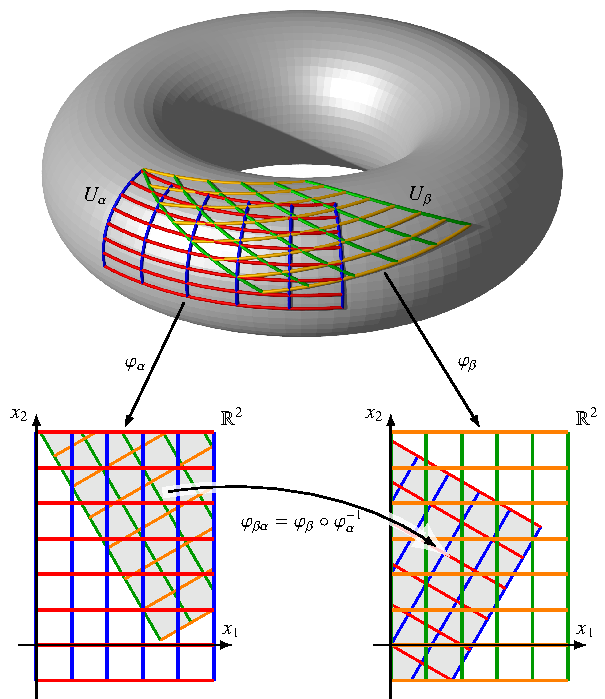
\includegraphics{chapters/020-koordinaten/images/karten.pdf}
\caption{Karten und Kartenwechsel auf einem Torus
\label{buch:koordinaten:fig:toruskarten}}
\end{figure}
%
%
% fig-koordinatenwechsel.tex
%
% (c) 2024 Prof Dr Andreas Müller
%
\begin{figure}
\centering
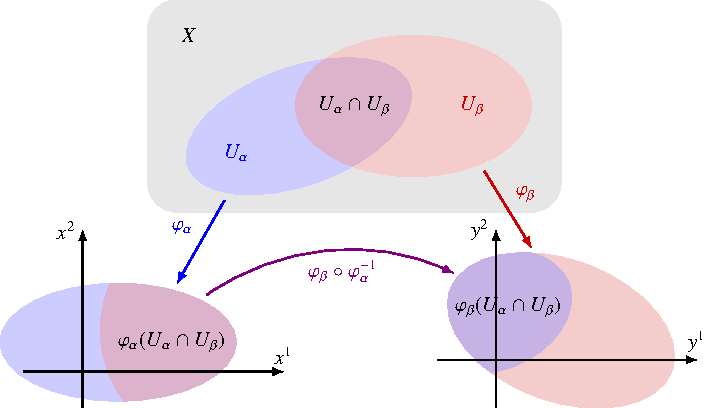
\includegraphics{chapters/020-koordinaten/images/koordinatenwechsel.pdf}
\caption{Koordinatenwechselabbildung $\varphi_\beta\circ\varphi_\alpha^{-1}$
zwischen zwei Karten $(U_\alpha,\varphi_\alpha)$ ({\color{blue}blau}) und
$(U_\beta,\varphi_\beta)$ ({\color{darkred}rot}).
\label{buch:koordinaten:diffmannig:fig:koordinatenwechsel}}
\end{figure}
%
Seien zwei Karten $(U_\alpha,\varphi_\alpha)$ und $(U_\beta,\varphi_\beta)$
gegeben derart, dass $U_\alpha\cap U_\beta$ nicht leer ist.
Auf der offenen Teilmenge $U_\alpha\cap U_\beta$ sind daher durch
die Abbildungen $\varphi_\alpha$ und $\varphi_\beta$ zwei
Koordinatensysteme gegegeben, die wir der Einfachheit halber wieder
mit den gleichen Symbolen bezeichnen\footnote{Genauer wäre, sie als
$\varphi_{\alpha|U_\alpha\cap U_\beta}$ und
$\varphi_{\beta|U_\alpha\cap U_\beta}$ zu bezeichnen, was jedoch
etwas schwerfällig ist.}.
Die Koordinatentransformation ist die Abbildung
\[
\varphi_\beta\circ\varphi_\alpha^{-1}
\colon
\varphi_\alpha(U_\alpha\cap U_\beta)
\to
\varphi_\beta(U_\alpha\cap U_\beta)
:
(x_\beta^1,\dots,x_\beta^n)
\mapsto
(x_\alpha^1,\dots,x_\alpha^n)
\]
(Abbildungen~\ref{buch:koordinaten:fig:toruskarten} und
\ref{buch:koordinaten:diffmannig:fig:koordinatenwechsel}).
Sie heisst der {\em Kartenwechsel} von der Karte $(U_\beta,\varphi_\beta)$
zur Karte $(U_\beta,\varphi_\beta)$.
\index{Kartenwechsel}%

\begin{definition}[Atlas]
Ein {\em Atlas} ist eine Familie $(U_\alpha,\varphi_\alpha)_{\alpha\in I}$
von Karten derart, dass die Kartenwechwechsel
$\varphi_\alpha\circ\varphi_\beta^{-1}$ Homöomorphismen
für alle $\alpha,\beta\in I$ sind, für die
$U_\alpha\cap U_\beta\ne \emptyset$ ist.
\end{definition}

\begin{definition}[differenzierbarer Atlas]
Ein {\em differenzierbarer Atlas} ist ein Atlas, dessen
Kartenwechsel differenzierbar sind.
\end{definition}

Zu einer stetigen Struktur auf $X$ gehört der Atlas $(X,\varphi)$,
wobei $\varphi$ alle Koordinatensysteme der stetigen Struktur druchläuft.
Ist sogar eine differenzierbare Struktur auf der Menge $X$ gegeben,
wie sie in
Definition~\ref{buch:koordinaten:koordinaten:definition:diffbareestruktur}
definiert worden ist, dann bilden die Karten $(X,\varphi)$, wobei
$\varphi$ die Koordinatensysteme der differenzierbaren Struktur
durchläuft, einen differenzierbaren Atlas.

Für die Kugeloberfläche ist es nicht möglich, ein Koordinatensystem
zu finden, welches die ganze Kugeloberfläche abdeckt.
Dieses Phänomen trifft auch bei vielen anderen geometrischen Formen ein.
Ein Atlas ermöglicht, sich bei der Konstruktion auf lokale Betrachtungen
in der Umgegung eines Punktes zu beschränken.

\begin{definition}[differenzierbare Mannigfaltigkeit]
Eine {\em differenzierbare Mannigfaltigkeit} ist eine Menge $X$, die überdeckt
wird von den Definitionsgebieten eines differenzierbaren Atlas auf $X$.
\index{differenzierbare Mannigfaltigkeit}%
\index{Mannigfaltigkeit!differenzierbar}%
\end{definition}

Nach dieser Definition müsste die zweidimensionale Kugeloberfläche eine
differenzierbare Mannigfaltigkeit sein.
Das nachfolgende Beispiel zeigt, wie ein differenzierbarer Atlas
für die Kugeloberfläche gefunden werden kann.

\begin{beispiel}
\label{buch:koordinaten:diffmannig:beispiel:stereographisch}
%
% fig-stereographisch.tex
%
% (c) 2024 Prof Dr Andreas Müller
%
\begin{figure}
\centering
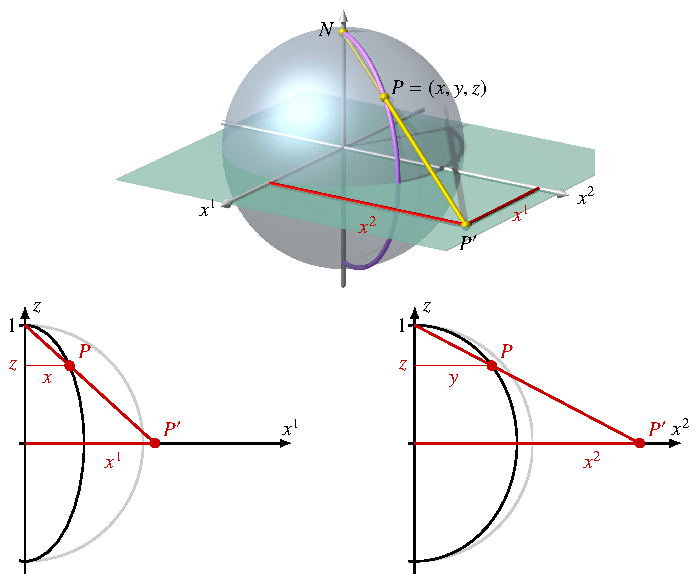
\includegraphics{chapters/020-koordinaten/images/stereographisch.pdf}
\caption{Stereographische Projektion eines Punktes $P$ mit Koordinaten
$(x,y,z)$ auf einer Kugeloberfläche auf die Äquatorebene mit den
Koordinaten $x^1$ und $x^2$.
\label{buch:koordinaten:diffmannig:fig:stereographisch}}
\end{figure}
%
Um zu zeigen, dass die zweidimensionale Kugeloberfläche
\[
S^2
=
\{
(x,y,z)\in\mathbb{R}^3
\mid
x^2 + y^2 + z^2 = 1
\}
\]
eine differenzierbare Mannigfaltigkeit ist, muss ein differenzierbare
Atlas konstruiert werden.
Dazu sind mindestens zwei Karten notwendig.
Wir konstruieren die Karten als stereographische Projektion von den
beiden Polen $N=(0,0,1)$ und $S=(0,0,-1)$ aus.
Als Definitionsbereich der Karten verwenden wir
\[
U_+
=
S^2\setminus \{ (0,0,1)\}
\qquad\text{und}\qquad
U_-
=
S^2\setminus \{ (0,0,-1)\}.
\]
Abbildung~\ref{buch:koordinaten:diffmannig:fig:stereographisch}
gestattet, die Kartenabbildung zu ermitteln.
Der Punkt $P$ mit den Koordinaten $(x,y,z)$ auf der Kugeloberfläche
wird auf den Punkt mit den Koordinaten $(x^1,x^2)$ abgebildet.
Der Strahlensatz besagt, dass
\[
\left.
\begin{aligned}
x : x^1
&=
(1-z) : 1
\\
y : x^2
&=
(1-z) : 1
\end{aligned}
\quad
\right\}
\qquad
\Rightarrow
\qquad
(x^1,x^2) = \frac{1}{1-z}(x,y).
\]
Auf die gleiche Weise kann man auch die stereographische Projektion vom
Südpol aus berechnen.
Als Kartenabbildungen verwenden wir daher
\[
\varphi_+
\colon
(x,y,z)
\mapsto
\frac{1}{1-z}
(x,y)
\qquad\text{und}\qquad
\varphi_-
\colon
(x,y,z)
\mapsto
\frac{1}{1+z}
(x,y).
\]



Die Umkehrabbildungen sind etwas kompliziert auszudrücken, werden
aber auch nicht wirklich benötigt, nur die Zusammensetzung
$\varphi_{\mp}\circ\varphi_{\pm}^{-1}$ müssen berechnet daraufhin
untersucht werden, ob sie differenzierbar sind.
%
% fig-stereowechsel.tex
%
% (c) 2024 Prof Dr Andreas Müller
%
\begin{figure}
\centering
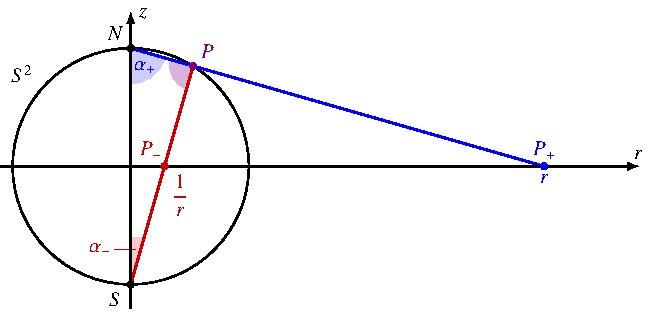
\includegraphics{chapters/020-koordinaten/images/stereowechsel.pdf}
\caption{Die stereographische Projektion $\varphi_+$ vom Nordpol
der Kugel aus bildet den Kugelpunkt $P$ auf den Punkt $P_+$ ab, die 
stereographische Projektion vom Südpol bildet ihn auf $P_-$ ab.
Die Kartenwechselabbildung $\varphi_-\circ\varphi_+^{-1}$ bildet $P_+$
auf $P_-$ ab.
Da $P$ auf dem Thales-Kreis über der Strecke $NS$ liegt, ist der Winkel
bei $P$ ein rechter Winkel und die Winkel $\alpha_+$ und $\alpha_-$
sind komplementär.
Es folgt, dass das Produkt der $r$-Koordinaten der Punkte $1$ ist.
\label{buch:koordinaten:diffmannig:fig:stereowechsel}}
\end{figure}
%
Die ist mit einem viel einfacheren geometrischen Argument möglich,
welches in Abbildung~\ref{buch:koordinaten:diffmannig:fig:stereowechsel}
erklärt wird.
Die Karte $\varphi_+$ bildet $P$ auf $P_+$ ab, $\varphi_-$ bildet
$P$ auf $P_-$ ab.
Da $P$ auf dem Thales-Kreis über der Strecke $NS$ liegt, ist der Winkel
$P$ ein rechter Winkel und die Winkel $\alpha_+$ und $\alpha_-$ sind
komplementär.
Die $r$-Koordinate von $P_-$ ist 
\[
\tan \alpha_-
=
\cot \alpha_+
=
\frac1{\tan\alpha_+}
=
\frac1{r}.
\]
Daraus lässt sich ableiten, dass die Kartenwechselabbildung
\[
\varphi_-\circ\varphi_+^{-1}
\colon
V_+\cap V_- \to V_-\cap V_+
:
(x^1_+,x^2_+)
\mapsto
\frac{1}{(x_+^1)^2 + (x_+^2)^2}(x_+^1,x_+^2)
\]
ist, die ganz offensichtlich differenzierbar ist, solange der 
Nenner nicht verschwindet.
\end{beispiel}

Der Begriff des Atlas erlaubt offenbar, lokale Eigenschaften, also
Eigenschaften, die sich in einer kleinen Umgebung eines Punktes 
feststellen lassen, mit Hilfe eines Koordinatensystems zu analysieren,
welches dafür am besten geeignet ist.
Alle anderen Koordinatensystem werden die Resultate ergeben, die mit
der Kartenwechselabbildung umgerechnet werden können.





\uebungsabschnitt

\aufgabetoplevel{chapters/020-koordinaten/uebungsaufgaben}
\begin{uebungsaufgaben}
\uebungsaufgabe{201}
\uebungsaufgabe{202}
\end{uebungsaufgaben}
\enduebungsabschnitt

